\documentclass[conference,comsoc,10pt]{IEEEtran}
\usepackage{cite}
\usepackage{amsmath,amssymb,amsfonts}
\usepackage{algorithmic}
\usepackage{graphicx}
\usepackage{textcomp}
\usepackage{xcolor}
\usepackage{array}
\usepackage[hyphens]{url}
\usepackage[colorlinks=true,urlcolor=black]{hyperref}
\def\BibTeX{{\rm B\kern-.05em{\sc i\kern-.025em b}\kern-.08em
    T\kern-.1667em\lower.7ex\hbox{E}\kern-.125emX}}
\newenvironment{conditions}
  {\par\vspace{\abovedisplayskip}\noindent\begin{tabular}{>{$}l<{$} @{${}={}$} l}}
  {\end{tabular}\par\vspace{\belowdisplayskip}}
\begin{document}

\hypersetup{
    colorlinks=true,
    linkcolor=blue,
    urlcolor=cyan,
}

\newcommand{\DOUBLEBLIND}{}   

\title{Practical usage of Zero-knowledge in different use-cases in blockchains} 

\author{\IEEEauthorblockN{Lukáš Častven}
    \IEEEauthorblockA{
        \textit{Faculty of informatics and information technologies}\\
        \textit{Slovak university of technology}\\
        Bratislava, Slovakia\\
        xcastven@stuba.sk
    }
}

\maketitle

\begin{abstract}
    Zero Knowledge Proofs (ZKP) are a cryptographic primitives which enables a
    validation of data without revealing the data itself, making it ideal for
    secure and private applications in blockchain networks. The focus of this
    study is a design and an implementation of a proof of concept Stealth
    Address scheme using ZKPs. This scheme will allow any sender to create a
    stealth address from recipients public data. Only the recipient has control
    over this address, yet it does not leak any information about who the
    recipient is.

    The core innovation of this work lies in replacing traditional elliptic
    curve cryptography, often used in stealth address schemes, with ZKPs. This
    substitution provides a trustless and privacy-preserving way to prove
    stealth address ownership without revealing sensitive details.

    This study advances the field of blockchain privacy by demonstrating the
    feasibility and advantages of incorporating ZKPs into stealth address
    schemes. It offers insights into the design of privacy-centric
    cryptocurrency solutions and highlights the potential of ZKPs to enhance
    anonymity and security on blockchains.

\end{abstract}

\begin{IEEEkeywords}
    cryptography, zero knowledge, privacy, cryptocurrency
\end{IEEEkeywords}

\section{Introduction}
    Zero Knowledge Proofs (ZKPs) are a powerful cryptography primitive. They allow
    for verification of a statement's truth without disclosing or in any way revealing
    the actual content of the statement. This characteristic is crucial for
    maintaining trust between parties while also preserving privacy \cite{goldreich1991proofs}.

    The concept of ZKPs was first introduced in a 1989 research paper, "The
    Knowledge Complexity of Interactive Proof Systems."\cite{Goldwasser1989}.
    This work describes how in traditional proofs, such as demonstrating a graph
    is Hamiltonian, more information is typically revealed than just the truth of
    the theorem. This paper develops a computational complexity theory focusing
    on the knowledge part within a proof. It introduces zero knowledge proofs,
    a novel concept where proofs only confirm the correctness of a proposition
    without exposing any extra knowledge.

    The paper focuses on interactive proofs, where a dialogue between a prover and
    a verifier occurs. In these interactive proofs, the prover aims to convince
    the verifier about the truth of a private statement, with a very small
    probability of error.

    With interactive proofs one can convince a probabilistic polynomial-time verifier
    of a \emph{PSPACE} statement's truth \cite{Shamir1992, Lund1992}. These proofs
    are pivotal in ZKPs, as they allow for the verification of a statement's truth
    without revealing the actual information or knowledge behind the statement,
    maintaining the principle of conveying no knowledge beyond the proposition's
    correctness.

    This thesis extends the application of ZKPs to the concept of stealth
    addresses in blockchain. Such as those outlined in Vitalik Buterin's article "An
    Incomplete Guide to Stealth Addresses."\cite{ButerinIncompleteGuide}, or
    in the Peter Todd's proposal to Bitcoin mailing list\cite{ToddStealthAddresses}.

    Blockchains, by their inherent design, make transactions publicly
    traceable. This transparency, while beneficial for certain use cases,
    compromises user privacy. Stealth addresses aim to solve this problem by
    obfuscating the identities of recipients, while still preserving owner
    control over them.
    They are critical for privacy on blockchains, allowing assets to
    be transferred without revealing the recipient's identity and making
    it difficult to link transactions to specific individuals.
    This makes it significantly harder to track an individual's
    financial activity on the blockchain, enhancing privacy and security.

\section{Background}
    This section begins with a demonstration of interactive proofs with goal to
    build up intuition behind interactive proofs \cite{Goldwasser1989,youtubeMOOCLecture1}.

    \subsection{Demonstration of an interactive zero knowledge proof}
        This section explains how Alice attempts to prove to Bob that she knows an
        algorithm, with which she computes some pair $(N, y)$, such that this pair is
        part of the quadratic residue language $QR$. Specifically, Alice needs to
        convince Bob that there exists an $x$, such that $y$ equals $x$ squared modulo $N$,
        effectively placing the pair $(N, y)$ within the $QR$ language, which includes all
        pairs where $y$ is a quadratic residue of $N$.

        Alice aims to prove to Bob that she knows an algorithm, which computes some pair $(N, y)$,
        such that this pair is part of the quadratic residue language $QR$ \cite{Goldwasser1989},
        where $QR$ is defined as:
        \[QR = \lbrace(N, y): \exists x, y \equiv x^2 \pmod{N}\rbrace\]

        The algorithm is as follows\cite{Goldwasser1989}:
        \begin{enumerate}
            \item Alice generates pair $(N, y)$,
            \item Alice picks a random $r$ such that $1 \leq r \leq N$ and $\gcd(r, N) = 1$,
                  and calculates $s \equiv r^2 \pmod{N}$,
            \item Alice sends Bob $s$,
            \item Alice asks Bob which value he wants. Either $\sqrt{s}$ or $\sqrt{sy}$, but he can not have both,
            \item Bob flips a coin and sends $b$ such that if coin landed on heads $b = 1$ else $b = 0$,
            \item If $b = 1$ Alice sends to Bob $z \equiv \sqrt{sy} \equiv r \sqrt{y} \pmod{N}$ else she sends $z \equiv \sqrt{s} \equiv r \pmod{N}$,
            \item Bob accepts if $z^2 = sy^b$.
        \end{enumerate}

        \begin{figure}[h!]
            \centering
            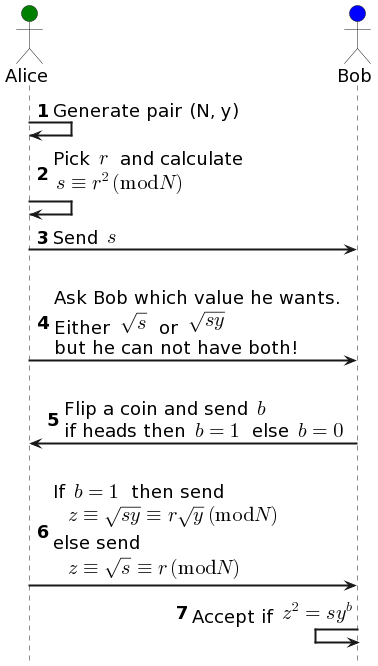
\includegraphics[scale=0.4]{../bachelor/assets/images/qr_ip.png}
            \caption{Interactive proof of language QR}
            \cite{Goldwasser1989, youtubeMOOCLecture1}
            \label{fig:qr_ip}
            \vspace{0.5cm}
        \end{figure}


        If Alice was a cheating prover, and she did not have the algorithm for
        generating pairs from $QR$, then the probability that Bob's coin toss favors
        Alice is one half. With one half probability Bob would ask cheating prover
        Alice to give him the equation she can not solve, because if the prover is
        cheating, she can not find the $\sqrt{s}$ and $\sqrt{sy}$. If she could,
        that would mean that she is not cheating.

        If the Alice's claim is true, Bob will accept. If Alice is not honest, and
        cheats, all verifiers will not accept with probability $P(Accept) = 0.5$.
        But this probability may not be satisfying enough. To make the probability
        that Alice is cheating smaller, Bob and Alice can start the interaction once
        again. This would lead to $P(Accept) = (0.5)^2$. They can redo the process
        as many times as they wish, resulting in $P(Accept) = (0.5)^k$ where $k$
        is how many different interactions they performed.

        Thanks to the randomness of the coin toss, there are $2^k$ possibilities how
        the interaction can go. Since Alice can not reliably predict what the random
        coin toss will yield, she must be ready to provide both equations. Thus Bob is
        convinced, that Alice is not cheating, with probability $P(Accept) = (0.5)^k$,
        and can accept the proof.

    \subsection{Overcoming limitation of an interactive proof}
        Interactive proofs require Alice to engage in a unique interaction with
        each individual verifier, which is not scalable or feasible for widespread
        application. Many ZKP protocols only require from the verifier a random input
        (for instance, a coin toss). Protocols, in which the verifier's role is
        generating some randomness and making it public are called public coin
        protocols \cite{Babai1988,Goldwasser1986}. The paper "How To Prove
        Yourself: Practical Solutions to Identification and Signature Problems"
        \cite{Fiat} by Fiat and Shamir demonstrates how these interactive public
        coin protocols can be efficiently transformed into non-interactive ones,
        offering a more scalable and practical solution for ZKPs.

        To transform a interactive public coin protocol into a non-interactive,
        Alice uses a random oracle which can provide a random coin toss based on some
        input. In practice the source of randomness of the random oracle is a
        cryptographic hash function, such as SHA256. Instead of sending messages back
        and forth between Alice and Bob, Alice provides to Bob a transformed
        transcript of the interaction. Since Bob's role in this interaction would only
        be generating random coin toss, Alice can in advance query the random oracle
        for this random value, and supply the message as an input to the query. The
        transcript string would look like this $(msg1, query(msg1), msg2, ...)$, where $query$ is
        the output from random oracle. This string and the public input of the proof
        can then be published and anybody, not just Bob, can validate this proof
        on their own.

        To illustrate, in scenario \ref{fig:interactive_coin}, where Alice
        sends only two messages and requires one random coin toss from Bob,
        Bob at the end can compute the validity of the proof from Alice with
        $validate(public\:input\:x,\:msg1,\:coin\:toss,\:msg2) = accept/reject$
        Then after applying Fiat-Shamir transform \ref{fig:non_interactive_coin},
        Alice only sends one message with the transcript string, and Bob can
        compute the validity of the proof like this
        $validate(public\:input\:x,\:msg1,\:query(msg1),\:msg2) = accept/reject$.

        \begin{figure}[h]
            \centering
            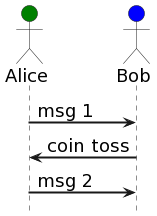
\includegraphics[scale=0.4]{../bachelor/assets/images/interactive_coin.png}
            \caption{Interactive public coin proof}
            \label{fig:interactive_coin}
            \cite{Goldwasser1986, youtubeMOOCLecture1}
            \vspace{0.5cm}
        \end{figure}

        \begin{figure}[h]
            \centering
            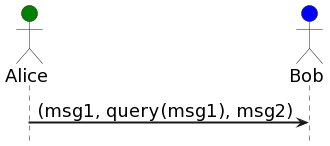
\includegraphics[scale=0.4]{../bachelor/assets/images/non_interactive_coin.png}
            \caption{Non-interactive public coin proof}
            \label{fig:non_interactive_coin}
            \cite{Fiat, youtubeMOOCLecture1}
            \vspace{0.5cm}
        \end{figure}

        Alice can publish the transcript string somewhere public, and anybody
        can rerun the interaction with the string in order to verify that Alice
        is lying or not.

    \subsection{Arithmetic circuit}

        While in theory any NP statement \cite{goldreich1991proofs} can be proven using
        interactive proofs, practical implementation requires specific definition and
        encoding of the statement. There are two main models of general computation,
        those are circuits and Turing machines. To trace the computation of a Turing
        machine, the representation needs to somehow handle memory and thus would accrue
        more complexity than if a circuit is used. To represent a statement as a
        circuit, an arithmetic circuit, a computation model composed of addition and
        multiplication operations, is used. This circuit encodes the statement into a
        form suitable for "zk-ifying", enabling the application of interactive proofs
        to a broader range of practical scenarios.

        Arithmetic circuits in a finite field $\mathbb{F}_p$ are used in majority
        of implementations. The arithmetic circuit is a function which takes
        $n$ elements from field $\mathbb{F}_p$ and returns one element from that field.

        \[AC: \mathbb{F}^n \rightarrow F \]

        The $AC$ can be represented as a directed acyclic graph, or a polynomial. For
        example, polynomial $x_1x_2 + (x_2 + x_3)^2$ represents the same circuit as this
        directed acyclic graph

        \begin{figure}[h]
            \centering
            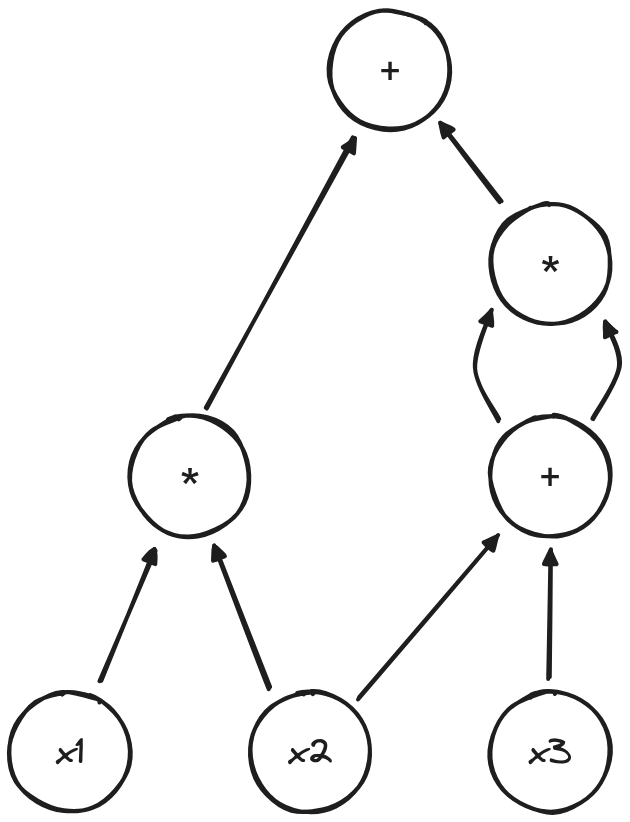
\includegraphics[scale=0.15]{../bachelor/assets/images/dag_example.png}
            \caption{Graph representation of arithmetic circuit}
            \label{fig:dag_example}
            \cite{youtuMOOCLecture3}
            \vspace{0.5cm}
        \end{figure}

        Another representation of an arithmetic circuits is called a Rank 1 Constraint
        System (R1CS). R1CS is a system of equations of a form $\alpha \times \beta = \gamma$,
        where $\alpha, \beta, \gamma$ are affine combinations of variables $w$ and $x$,
        where $w$ is a witness (private inputs) and $x$ is a public inputs.

        These are some examples of R1CS equations:
        \begin{displaymath}
            \begin{array}{l}
                (w_1 + x_3) \times (w_2 - x_1 + 1) = w_3 \\
                w_1 \times w_1 = x_1                     \\
                w_1 \times x_2 = w_3
            \end{array}
        \end{displaymath}

        And here is an example of a invalid R1CS equations, because they are not linear
        combinations of variables $w$ and $x$:

        \begin{displaymath}
            \begin{array}{l}
                w_1 \times x_3 \times w_2 = w_3 \\
                w_1 \times w_1 \times w_1 = x_1 \\
                w_1 \times x_2 + w_3 = w_4 \times w_5
            \end{array}
        \end{displaymath}

        To constrain the operation $w_1^3 = x_1$ in R1CS, there must be two equations, with
        a new intermediary variable $w_2$:

        \begin{displaymath}
            \begin{array}{l}
                w_1 \times w_1 = w_2 \\
                w_1 \times w_2 = x_1
            \end{array}
        \end{displaymath}

    \subsection{SNARKs}

        After defining an arithmetic circuit, it can be transformed into a SNARK,
        a Succinct Non-interactive ARgument of Knowledge. The succint part means that
        the size of the proof must be sublinear in size of witness (when talking about
        strong succinctness, the proof size is logarithmic in size of circuit), and
        the verification must be sublinear in size of circuit and linear in size of
        public input (when talking about strong efficiency, the verification time is
        logarithmic in size of circuit and linear in size of public input).
        A SNARK is a tripple of algorithms $(Setup, Prove, Verify)$\cite{Groth16}.

        \begin{enumerate}
            \item $Setup$ takes
                the arithmetic circuit $C(x, w) \rightarrow \mathbb{F}$, where $x$ is a public
                input (from $\mathbb{F}^n$) and $w$ is a witness (from $\mathbb{F}^m$), and
                is preprocessed, which creates public parameters $pp$ (prover's parameters)
                and $vp$ (verifier's parameters). This setup process is what enables the
                proof to be logarithmic in size of circuit. It is a summary of the circuit,
                so the verifier does not need to know the whole circuit, just the summary,
            \item $Prove$ algorithm takes the prover's parameters $pp$, public input $x$,
                witness $w$ and creates a proof $\pi$ which proves that $C(x, w) = 0$.
            \item $Verify$ algorithm takes the verifier's parameters $vp$, public input $x$ and
                proof $\pi$ and returns $accept/reject$.
        \end{enumerate}

        SNARKS combine two cryptographic primitives, a functional commitment scheme
        and an interactive oracle proof, in order create and verify the proof.
        Functional commitment scheme is a cryptographic primitive, which allows the
        prover to commit to a function $f$ and the verifier can query the commitment and
        prover must provide the evaluation of the function $f$ at the queried point,
        and a proof that the evaluation is correct.
        Interactive oracle proofs begin with a vector of function commitments.
        Verifier can interactively query any of the commitments and prover must
        provide the evaluation of the function at the queried point, and a proof
        that the evaluation is correct\cite{SassonIOPs}.


    \subsection{Stealth addresses}

        The concept of stealth addresses was introduced in 2014 by Peter Todd \cite{ToddStealthAddresses}.
        They were based on elliptic curve cryptography and enabled senders to
        send funds to a recipient without leaking the recipient's identity to
        the public. Only the recipient can then prove that they own the stealth
        address, and can spend the funds from it. Recipients must publish a meta
        stealth address, from which senders can derive a new stealth address.
        This new stealth address is not be linked to the meta stealth address,
        and thus the recipient's identity is protected.

        This study showcases how to swap elliptic curve cryptography for ZKPs.
        They can be used to prove that the recipient owns the stealth address, and
        thus can spend the funds. The proof can be sent from any address, but only
        the recipient can generate it, because only he/she knows the private data
        that is required to generate the proof. The zero knowledge property of the
        proof ensures that the recipient's identity is not revealed.

    \section{Related Work}

        With the growth of cryptocurrencies, ZKPs have gained a substantial popularity
        not only in academic circles, but also in the startup and venture capital
        ones. Many researchers are studying this field and it is not considered 
        as a cryptography for nerds anymore.

        On the other hand, there are not many contributions to the stealth address
        ecosystem. There are two protocols on Ethereum that implement stealth addresses.
        First one is called Umbra\cite{umbra}, and it is based on elliptic curve
        cryptography.

        The second one is called Nocturne\cite{nocturne}. The protocol is a mix of
        elliptic curve cryptography and ZKPs with few intermediate smart contracts.
        In this protocol you lock your funds in the Nocturne ecosystem, in which
        new stealth addresses are created with Elliptic curve stealth addresses scheme,
        and you access your funds by submitting ZKPs. However according to their
        \href{https://twitter.com/nocturne_xyz/status/1749510390906511693}{Twitter post}
        they are discontinuing their protocol.

\section{Solution Design}

    The core principle behind the solution is that both
    receiver and sender generate a random value. These two values can then
    be used to prove to a stealth address that whoever owns these values
    is the owner of the stealth address, and can control it. High level
    overview of the whole process is shown in Figure \ref{fig:high-level-flo}.

    Bob, as a receiver, publishes the hash of his random value to a public
    registry. With this hash he also publishes his public key, which corresponds
    to his private key. This tuple is Bob's meta stealth address, visualized in Figure
    \ref{fig:bobs-meta-address}.

    \begin{figure}[h]
        \centering
        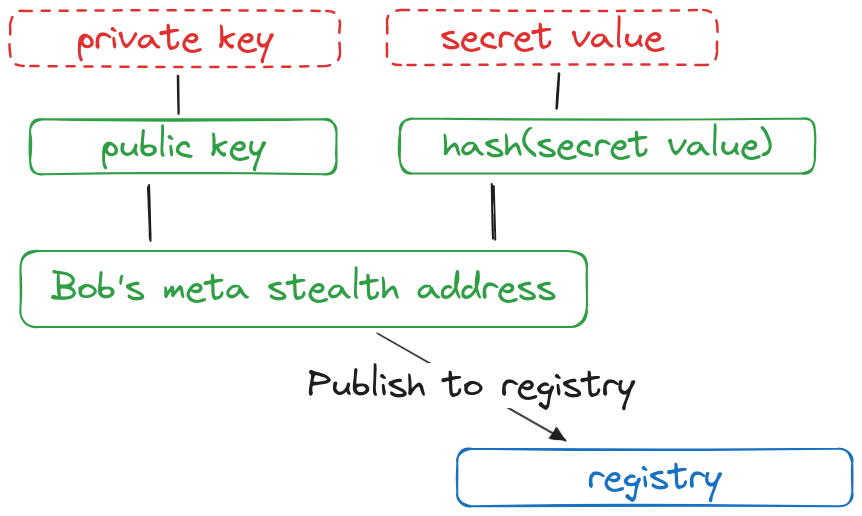
\includegraphics[scale=0.20]{./assets/images/meta-stealth-address.png}
        \caption{Bob's Meta Stealth Address}
        \label{fig:bobs-meta-address}
    \end{figure}

    When Alice wants to send funds to Bob, she finds his meta stealth address
    in the public registry, generates her own random value and hashes it together
    with Bob's hash to create a code. Then she deploys a new stealth wallet
    contract with this code in it, and amount of funds that she wanted to send
    to Bob. After that, she encrypts her random value with Bob's public key,
    this encrypted value is called ephemeral key. Alice publishes it to a
    public registry. This whole process is depicted in Figure \ref{fig:sending-funds}. 

    \begin{figure}[h]
        \centering
        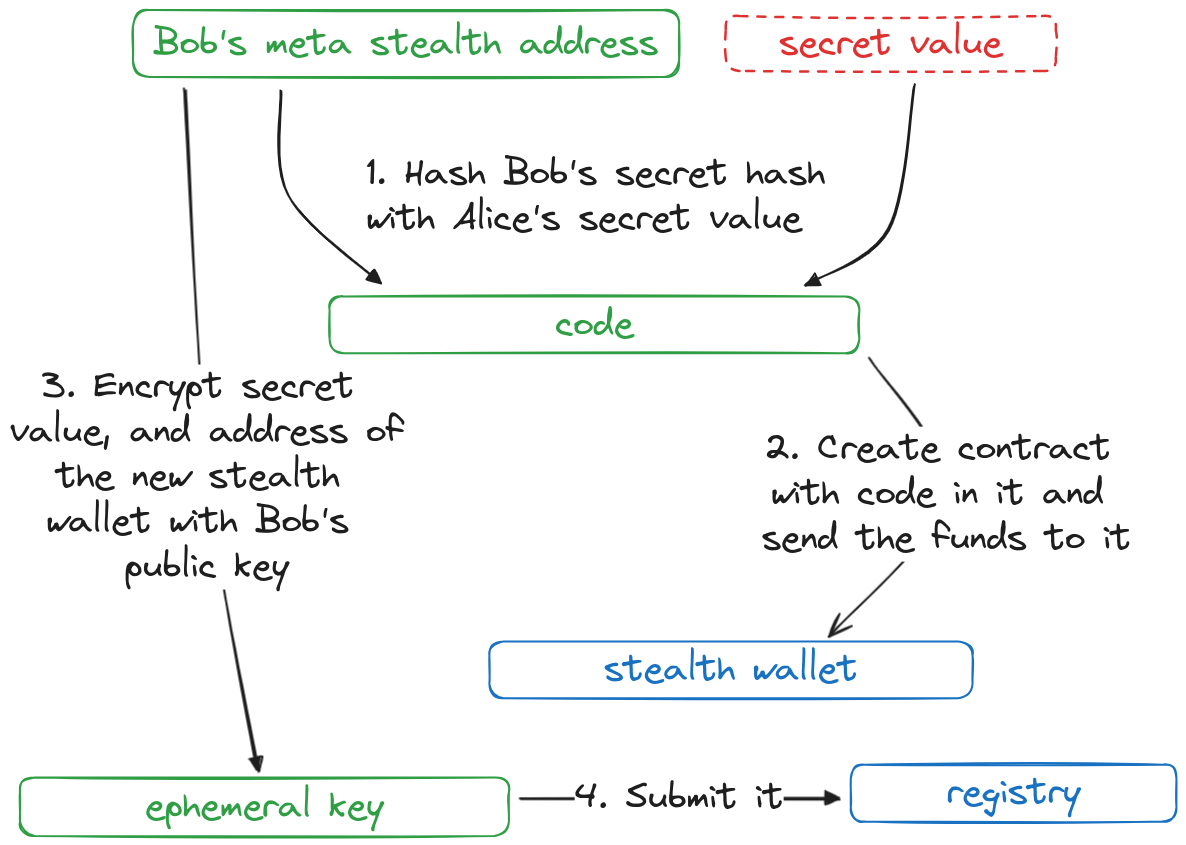
\includegraphics[scale=0.17]{./assets/images/sending-funds.png}
        \caption{Alice sends funds}
        \label{fig:sending-funds}
    \end{figure}

    Bob then scans the registry, tries to decrypt ephemeral keys. When the
    decryption is successful, Bob can save the decrypted Alice's secret value
    and the address of the corresponding stealth wallet.

    \begin{figure}[h]
        \centering
        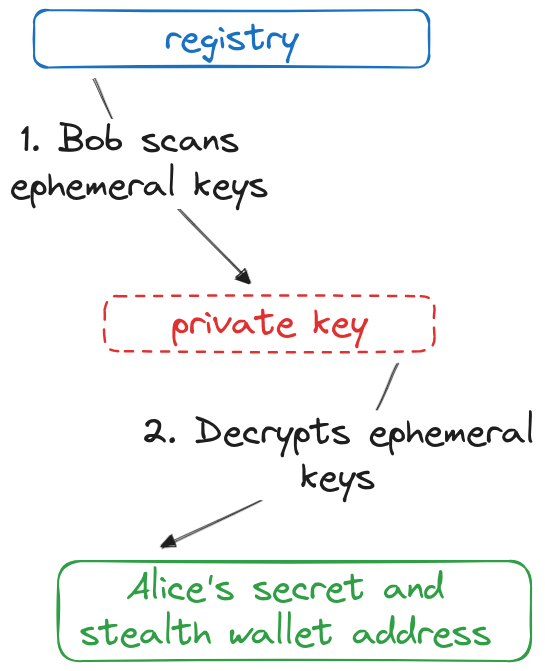
\includegraphics[scale=0.25]{./assets/images/scanning-ephemeral-keys.png}
        \caption{Bob scans ephemeral keys}
        \label{fig:scanning-ephemeral-keys}
    \end{figure}

    To use the funds, Bob must generate a ZK proof and submit it to the stealth
    wallet. This proof proves that Bob knows Alice's random value
    and his own random value, such that
    \[ code = hash(hash(Bob's\:value),\:Alice's\:value) \]
    where $code$ is the one submitted by Alice into the stealth wallet contract.

    \begin{figure}[h]
        \centering
        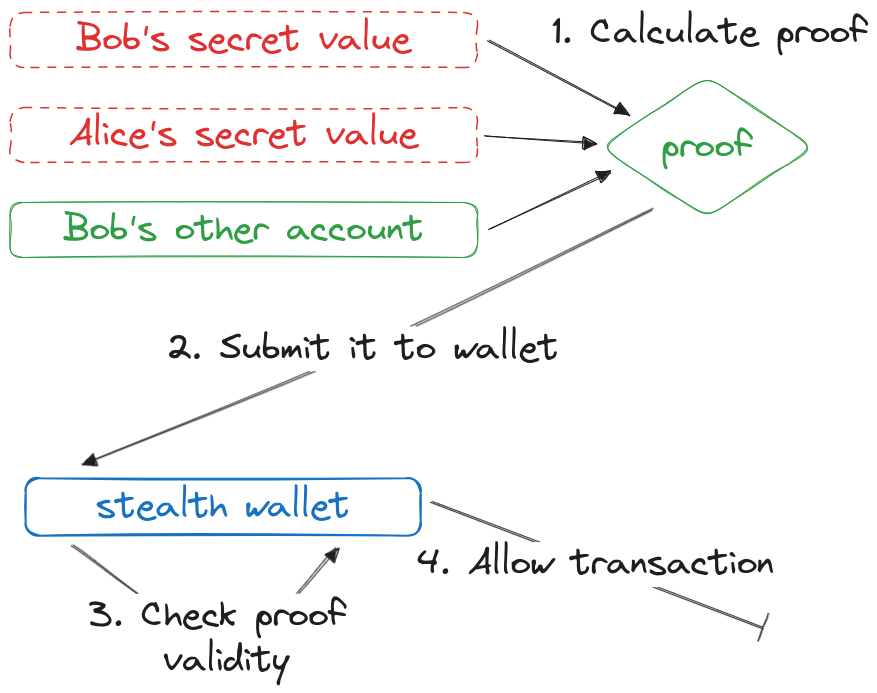
\includegraphics[scale=0.25]{./assets/images/interating-with-wallet.png}
        \caption{Bob's interaction with wallet}
        \label{fig:wallet-interaction}
    \end{figure}

    To prevent others from copying the proof when Bob sends it in a transaction,
    and gaining control over wallet with a higher fee transaction, the proof
    must also verify the sender of the transaction. In the proof, there must
    be a check that the address with which Bob wants to interact with the
    stealth wallet is the one sending the transaction. Without this check a malicious
    actor could copy the proof and send a transaction with higher fee, which would
    give him access to the wallet sooner, because it would be placed higher in
    the block. Since only Bob knows both secret values and an address from which
    he will be sending transaction, only he can create a valid proof and thus
    interact with the wallet.

    \begin{figure}[h]
        \centering
        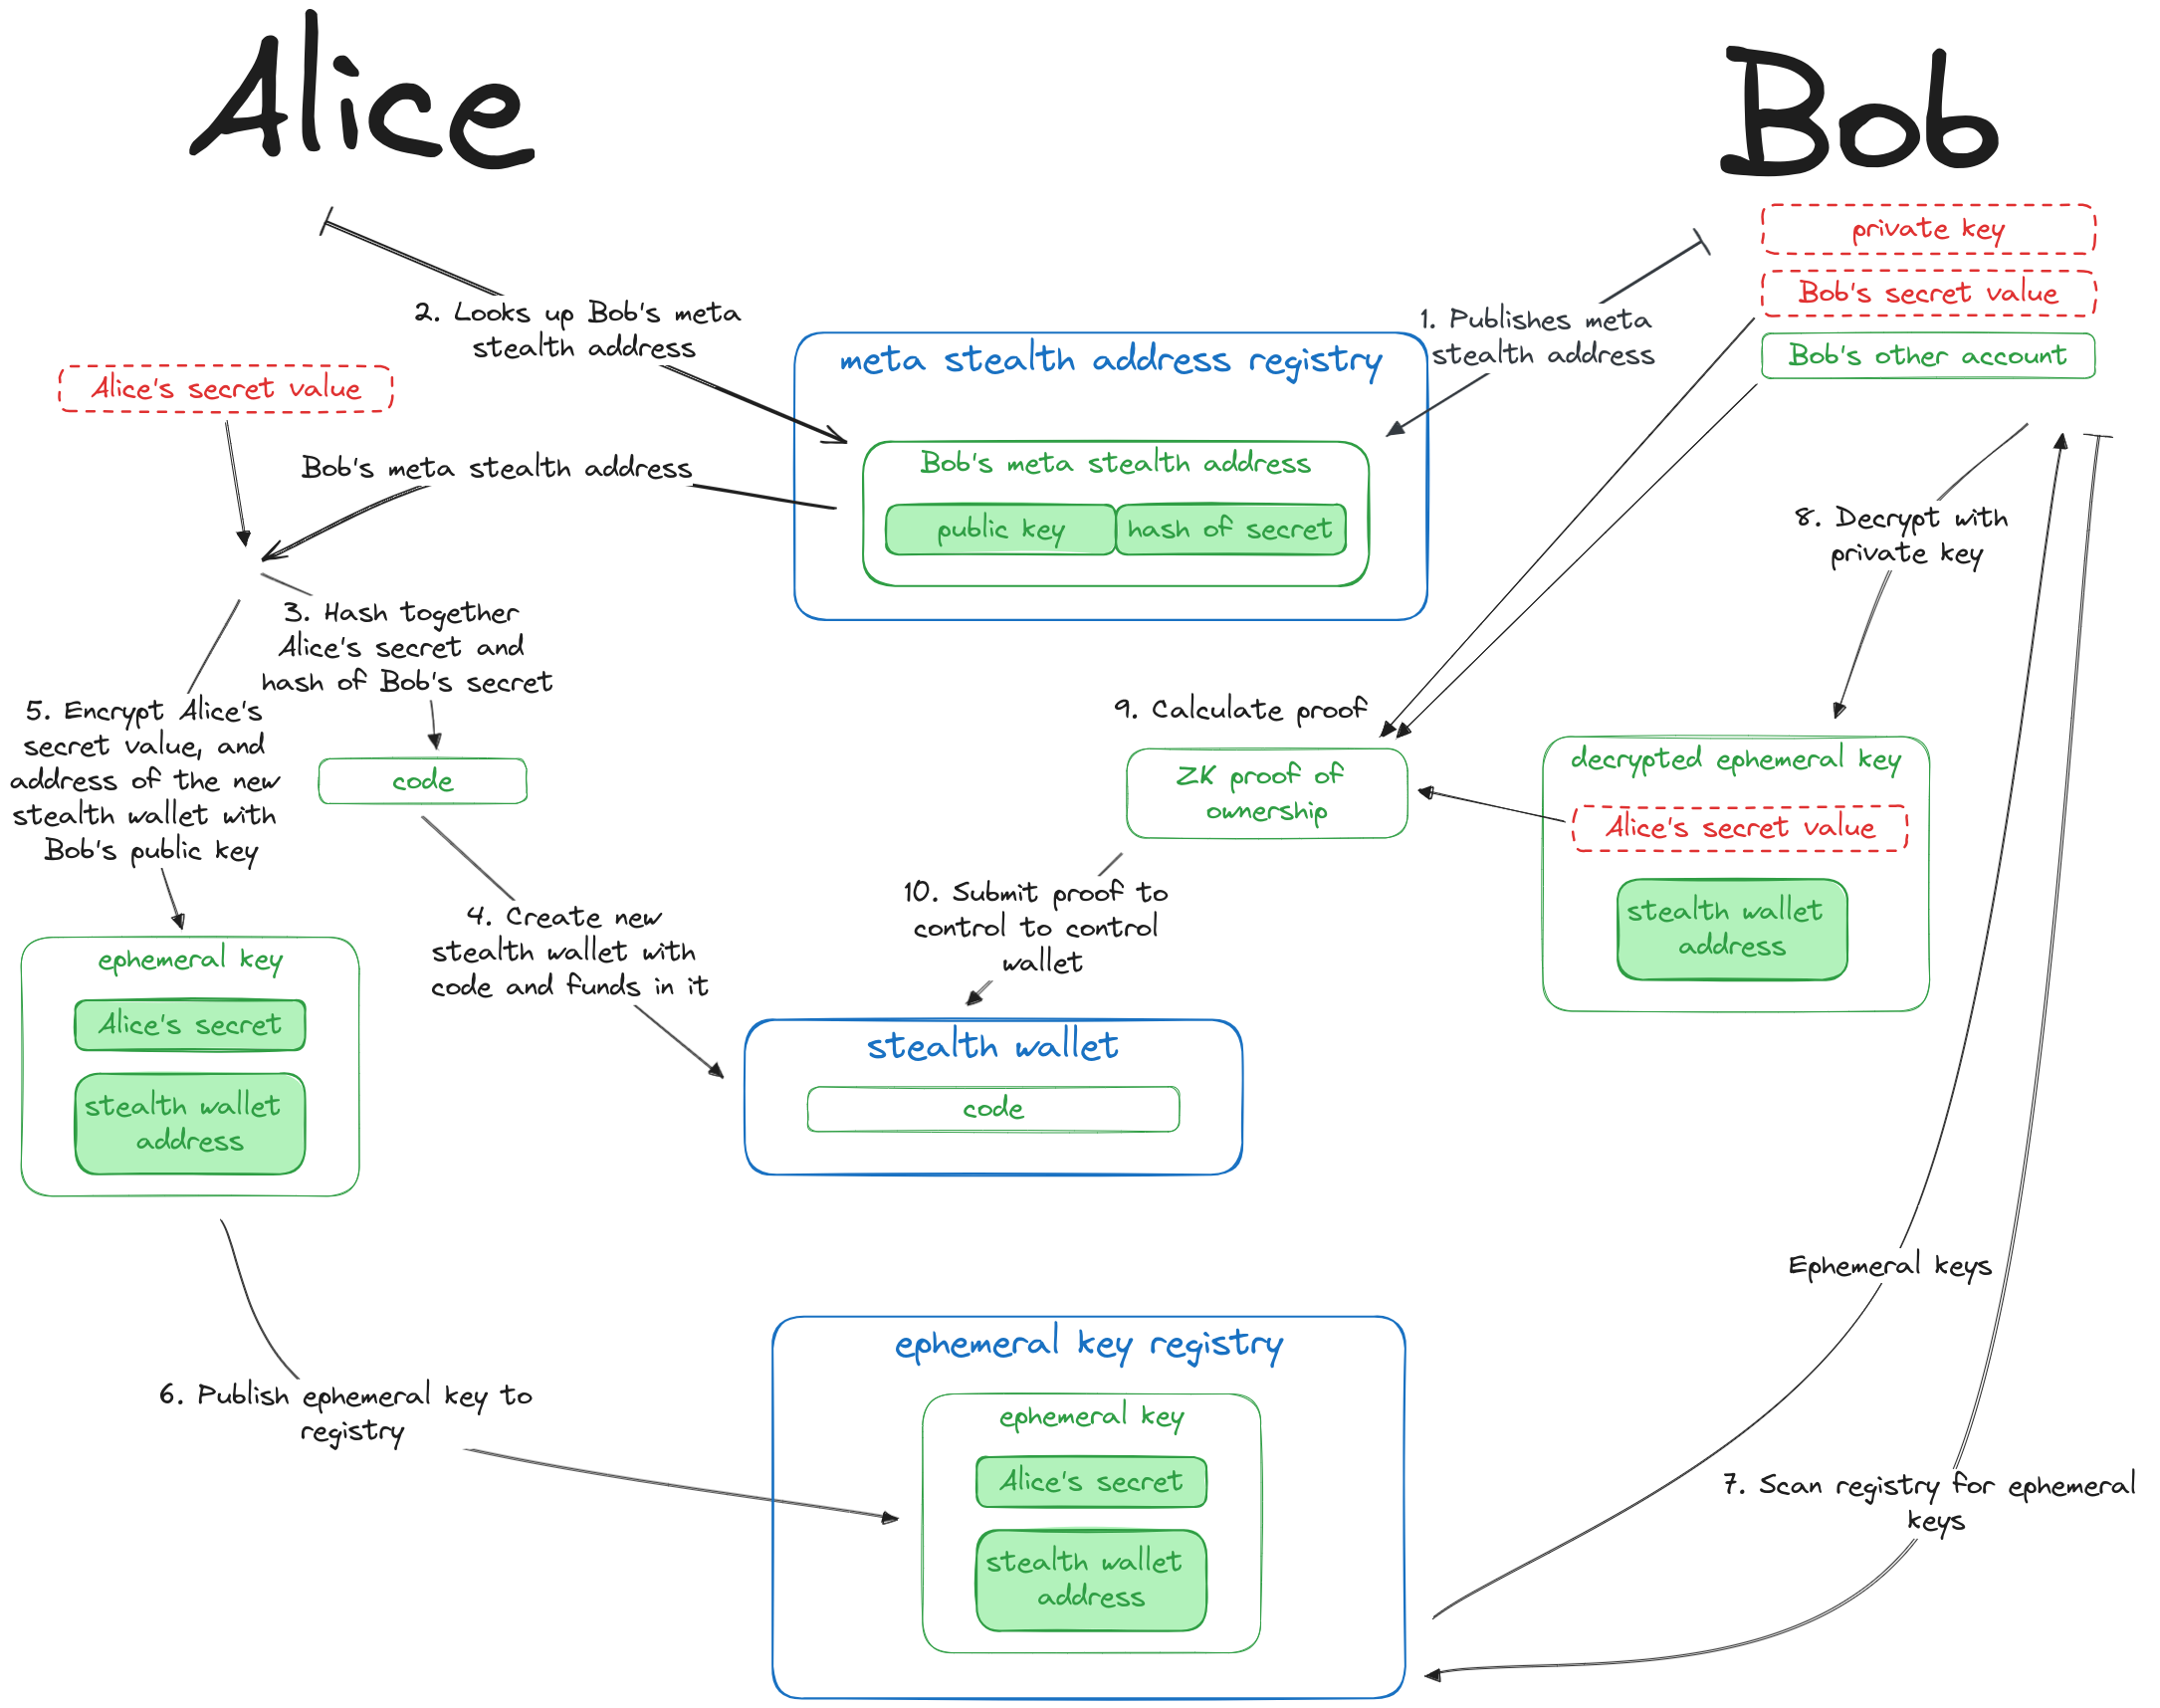
\includegraphics[scale=0.11]{../bachelor/assets/images/high-level-flow.png}
        \caption{High level overview}
        \label{fig:high-level-flow}
    \end{figure}

\section{Discussion on security}

    This section discuses the security properties of the proposed stealth address
    ZK-SNARK scheme. A secure scheme should ensure both the confidentiality
    of recipient's identity and the recipient's exclusive control over their
    stealth addresses. The scheme is analyzed under various assumptions
    regarding cryptographic primitives and the underlying protocols.

    \textbf{Assumptions}
    \begin{itemize}
        \item \textbf{Groth16}: The scheme relies on the completeness, soundness,
            and zero-knowledge properties of the Groth16 proof system.
        \item \textbf{Trusted Setup}: The security of generated public parameters
            depends on the integrity of the trusted setup process. The original
            parameters must be securely destroyed.
        \item \textbf{Hash Function}: A collision-resistant hash function is
            essential to prevent adversaries from finding alternative values
            that could mimic a legitimate owner's secret.
        \item \textbf{Elliptic Curve Cryptography}: The security of Secp256k1 is
            assumed.
        \item \textbf{Secrecy of Secret Values}: Both the recipient's (Bob's)
            and the sender's (Alice's) secret values must remain protected
            to ensure the scheme's integrity.
    \end{itemize}

    Under these assumptions, the Stealth Address ZKP Scheme enables the
    secure and anonymous transfer of assets to a recipient. The recipient
    has guaranteed exclusive control over their stealth addresses.

    However, it is important to highlight the following potential weak points:
    \begin{itemize}
        \item \textbf{Compromised Trusted Setup}: If the original parameters from
            Groth16's setup are not destroyed, false proofs could be generated.
        \item \textbf{Collision in Hash Function}: If a collision is found in
            the hash function, funds from a single stealth address could be at
            risk.
        \item \textbf{Exposure of Secret Values}: Leaking both of the
            recipient's secret and the sender's secret can lead to
            unauthorized access or loss of funds.
    \end{itemize}

\section{Evaluation}

    The stealth address ZKP scheme successfully enables private transactions.
    It effectively hides the recipient's identity, yet he/she still has control
    over received funds, thanks to zero-knowledge proofs. They also ensuring no
    direct link between transactions and the recipient can be created.
    Simultaneously, only the intended recipient can generate the necessary
    ZKPs to access funds, through possessing both secret values. This
    guarantees exclusive control over stealth addresses.

    The scheme offers a compelling solution for privacy-centric cryptocurrency
    use cases. While security considerations must be addressed more thoroughly, it
    demonstrates the potential of ZKPs in enhancing blockchain anonymity.

\section{Conclusion and Future Work}

    This study opens up few avenues for future research and improvements
    to this proof of concept:

    \begin{enumerate}
        \item Adding functionality, such as fractional withdrawals, ERC20 token transfers,
        \item How to setup initial parameters of a circuit to achive trustworthiness
                and security,
        \item Formal proof of security and soundness of proposed solution,
        \item Smart contract optimizations via gas optimizations in the Solidity code,
        \item Exploring different ZKP proof systems with comparisons and benchmarks,
        \item Incorporate recoverability into stealth wallets.
    \end{enumerate}

    The work investigated the application of Zero-Knowledge Proofs (ZKPs)
    in stealth addresses schema on Ethereum. The primary research
    goal was to design and implement a proof of concept stealth address schema
    which utilizes ZKPs to achieve privacy of transactions.
    The solution aimed to protect a recipient's identity (Bob) while enabling
    a sender (Alice) to transfer funds without any way of identitying the
    recipient.

    The implementation demonstrates the core concept of a
    ZKP-based stealth address schema. Senders deploy stealth wallets
    associated with a code derived from a combination of their secret value
    and the recipient's hashed secret. The recipient can generate ZKPs,
    proving knowledge of both secret values, to withdraw funds from their
    corresponding stealth wallets. The design also ensures that proofs can
    only be valid when submitted by the specific recipient who owns both
    secret values. It is important to note that the current implementation
    serves as a proof of concept, and further development
    would be necessary for real-world deployment as a full-featured wallet. 

    In conclusion, this research work demonstrates the feasibility and
    advantages applying ZKPs into stealth address schema. The privacy
    protection provided by ZKPs in this context highlights a promising
    direction for strengthening anonymity in cryptocurrency transactions.

\begin{thebibliography}{00}
    \bibitem{goldreich1991proofs} O. Goldreich, S. Micali, and A. Wigderson, “Proofs that yield nothing but their validity or all languages in NP have zero-knowledge proof systems,” Journal of the ACM (JACM), vol. 38, no. 3, pp. 690–728, 1991.
    \bibitem{Goldwasser1989} S. Goldwasser, S. Micali, and C. Rackoff, “The Knowledge Complexity of Interactive Proof Systems,” SIAM Journal on Computing, vol. 18, no. 1, pp. 186–208, Feb. 1989, doi: 10.1137/0218012.
    \bibitem{Shamir1992} A. Shamir, “IP = PSPACE,” Journal of the ACM, vol. 39, no. 4, pp. 869–877, Oct. 1992, doi: 10.1145/146585.146609.
    \bibitem{Lund1992} C. Lund, L. Fortnow, H. Karloff, and N. Nisan, “Algebraic methods for interactive proof systems,” Journal of the ACM, vol. 39, no. 4, pp. 859–868, Oct. 1992, doi: 10.1145/146585.146605.
    \bibitem{Fiat} A. Fiat and A. Shamir, “How To Prove Yourself: Practical Solutions to Identification and Signature Problems,” in Lecture Notes in Computer Science, Springer Berlin Heidelberg, pp. 186–194. doi: 10.1007/3-540-47721-7\_12.
    \bibitem{Groth16} J. Groth, “On the Size of Pairing-Based Non-interactive Arguments,” in Lecture Notes in Computer Science, Springer Berlin Heidelberg, 2016, pp. 305–326. doi: 10.1007/978-3-662-49896-5\_11.
    \bibitem{ButerinIncompleteGuide} An incomplete guide to stealth addresses — vitalik.eth.limo. https://vitalik.eth.limo/general/2023/01/20/stealth.html. [Online]. Available: https://vitalik.eth.limo/general/2023/01/20/stealth.html
    \bibitem{ToddStealthAddresses} [Bitcoin-development] Stealth Addresses — lists.linuxfoundation.org. https://lists.linuxfoundation.org/pipermail/bitcoin-dev/2014-January/004020.html. [Online]. Available: https://lists.linuxfoundation.org/pipermail/bitcoin-dev/2014-January/004020.html
    \bibitem{youtubeMOOCLecture1} ZKP MOOC Lecture 1: Introduction and History of ZKP — youtube.com. \url{https://www.youtube.com/watch?v=uchjTIlPzFo&list=PLS01nW3Rtgor_yJmQsGBZAg5XM4TSGpPs}. [Online]. Available: \url{https://www.youtube.com/watch?v=uchjTIlPzFo&list=PLS01nW3Rtgor_yJmQsGBZAg5XM4TSGpPs}
    \bibitem{Babai1988} L. Babai and S. Moran, “Arthur-Merlin games: A randomized proof system, and a hierarchy of complexity classes,” Journal of Computer and System Sciences, vol. 36, no. 2, pp. 254–276, Apr. 1988, doi: 10.1016/0022-0000(88)90028-1.
    \bibitem{Goldwasser1986} S. Goldwasser and M. Sipser, “Private coins versus public coins in interactive proof systems,” 1986. doi: 10.1145/12130.12137.
    \bibitem{youtuMOOCLecture3} ZKP MOOC Lecture 3: Programming ZKPs — youtu.be. \url{https://youtu.be/UpRSaG6iuks?si=CeuQSD6N8PslfNJa}. [Online]. Available: \url{https://youtu.be/UpRSaG6iuks?si=CeuQSD6N8PslfNJa}
    \bibitem{SassonIOPs} E. Ben-Sasson, A. Chiesa, and N. Spooner, Interactive Oracle Proofs. Cryptology ePrint Archive, Paper 2016/116, 2016. [Online]. Available: https://eprint.iacr.org/2016/116
    \bibitem{umbra} Umbra — app.umbra.cash. https://app.umbra.cash/. [Online]. Available: https://app.umbra.cash/
    \bibitem{nocturne} Nocturne — nocturne.xyz. https://nocturne.xyz/. [Online]. Available: https://nocturne.xyz/

\end{document}
